% #############################################################################
% This is Chapter 3
% !TEX root = ../main.tex
% #############################################################################
% Change the Name of the Chapter i the following line
\fancychapter{European Normative Acts}
% The following line allows to ref this chapter
\label{chap:euacts}

Every action taken by the \ac{EU} is based on treaties. They are the starting point for \ac{EU} law and are hence referred to as primary law. The \ac{EU} is limited by the principle of conferral, meaning that the \ac{EU} can ``only act within the limits of the competences conferred upon it by the Member States int the Treaties to attain the objectives set out therein. Competences not conferred upon the Union in the Treaties remain with the Member States.''\cite{TEU_Art5_2016} 

The body of law that comes from the principles and objectives of the treaties is known as secondary law. These include legislative and non-legislative acts.
Currently there are five types of juristic acts, including regulations, directives, decisions, recommendations and opinions\footnote{\label{fn:euCom}Types of \ac{EU} law can be found here: \url{https://commission.europa.eu/law/law-making-process/types-eu-law_en}}.
\begin{itemize}
    \item Regulations - Legal acts that are binding in their entirety. They are directly and uniformly applicable to all \ac{EU} member states as soon as they enter into force, without needing to be transposed into national law.
    \item Directives - Set binding objectives upon \ac{EU} member states to achieve a certain result, but leave them free to choose how to achieve these objectives. 
    \item Decisions - Binding in their entirety, can specifies those to whom it is addressed, being binding only on them.
    \item Recommendations - Non-binding. They allow the \ac{EU} institutions to make their views known and to suggest a line of action without imposing any legal obligation.
    \item Opinions - Also non-binding, opinions allow \ac{EU} institutions to make a statement without imposing any legal obligation.
\end{itemize}

As a practical example, \ac{eIDAS2}, \ac{CSA} and \ac{DORA} are regulations, hence having a legal binding that applies uniformly across all \ac{EU} member states.\ac{NIS2} on the other hand, as a directive, sets goals that member states must achieve in the way they see fit, allowing the country to implement measures that lead to these objectives through national law.

\section{Regulation as an Architectural Constraint}

Regulation functions as a major architectural driver. As noted by Bolinhas\cite{Pbol}, ``the legal framework is a significant constraint for all businesses, notably when dealing with an increasing number of regulations and directives'' \cite{practiceEnterpriseModelling}. These constraints may affect different dimensions. Regulations like \ac{DORA} mandate the creation of specific organizational units, or roles, such as the Lead Overseer. This effectively ``draws'' the organizational map, implementing a structural constraint. These constraints also exist in a behavioural form, since legislations describe rules, which are fundamentally rights and obligations \cite{Breaux2007} describing what can and cannot be done. Other constraints, like data protection laws, impose constraints on how to handle business objects, defining how data can be stored, for how long and who has access rights to the data. \ac{DORA} also imposes a type of ``supply chain'' dependencies, requiring financial organizations to audit and constrain their third-party service providers \cite{DORA}.

Organisations may be subject to several interacting legal requirements, whose implementation can constrain architectural choices. \ac{AD}s can make these constraints and dependencies explicit and support comparison between implementation alternatives within the applicable legal boundaries. Resolving conflicts between regulations is outside the scope of the demonstrations presented here, which examine stakeholder-specific representations of \ac{DORA}.

% #############################################################################
\section{Legislation Structure} 
\label{sec:legisStruc}

Identifying the structure of an \ac{EU} legal act is necessary for locating the provisions represented by architectural requirements. The Interinstitutional Style Guide describes the principal components of an act\footnote{\label{ft:howToReadEULaw}Structure and a guide on how to read \ac{EU} law can be found on: \url{https://fabianbohnenberger.com/2024/04/10/how-to-read-eu-law/comment-page-1/}}:\cite{EUStyleGuideLegalActStructure}
\begin{enumerate}
    \item \textbf{Title};
    \item \textbf{Preamble}(Citations, Recitals, Solemn Forms);
    \item \textbf{Enacting Terms} (and Annexes).
\end{enumerate}

Presenting each structural part in order, and starting with the title, that already holds a lot of important information:
\begin{itemize}
    \item The type of act (referenced in \ref{chap:euacts});
    \item Institution(s) that adopted the act (Parliament, Council, Commission);
    \item Whether the act is amending any existing law, and lists all the acts that are amended  or repealed;
    \item If it is an implementing or delegated act;
    \item The date of adoption;
    \item The reference number of the act;
    \item Indication of the broad policy area (\ac{EU}, Common Foreign and Security Policy, or European Atomic Energy Community);
    \item Outlines the subject/contents of the act, sometimes also providing a short title added at the end.
\end{itemize}
Figure \ref{fig:nis2Title} presents the title of the directive \ac{NIS2}, which unlike \ac{DORA} provides all of the informations listed above.


\begin{figure}
  \centering
  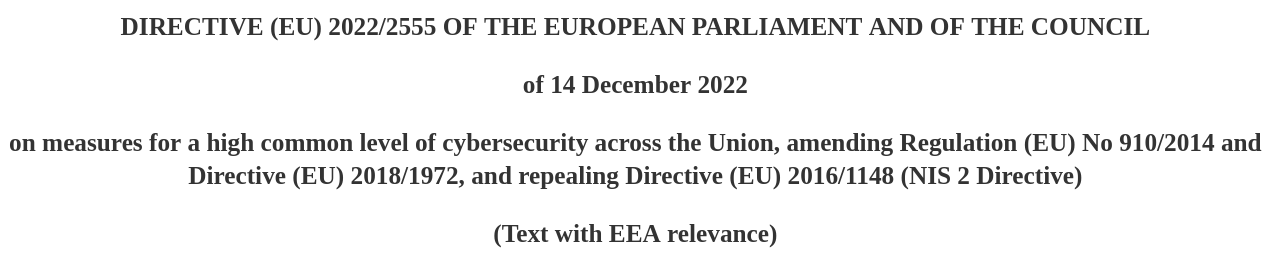
\includegraphics[width=1\textwidth]{Images/Nis2Act.png}
  \caption{Title of the \ac{NIS2} directive}
  \label{fig:nis2Title}
\end{figure}

Next to the title in the legal text is were the preamble is found. It encapsulates everything between the title and the ``Enacting terms''. The preamble is made up of three main elements: citations, recitals and solemn forms.

\begin{itemize}
    \item \textbf{Citations} establish the legal authority of the \ac{EU} and detail the legislative procedure used for adoption, relying on standardized language that generally starts with “Having regard to...”. \ac{DORA} establishes the necessary legal authority by citing Article 114 of \ac{TFEU} in the preamble (``Having regard to the Treaty on the Functioning of the European Union, and in particular Article 114 thereof'')\cite{DORA}; 
    \item \textbf{Recitals} then supply the statement of reasons, specifying the measure’s goals, the need for \ac{EU} action, and the reasoning behind the chosen regulatory method. These are numbered and either begin with the word ``whereas'', or are place after a single ``whereas'' before the enumeration begins. They provide interpretative value but are non-binding.
    \item \textbf{Solemn forms} act as grammatical brackets, turning the entire preamble into a single continuous sentence. It opens by identifying the enacting institutions (e.g., “THE EUROPEAN PARLIAMENT AND THE COUNCIL OF THE EUROPEAN UNION,”), encompasses the citations and recitals, and concludes with the enacting formula: “HAVE ADOPTED THIS REGULATION:”.
\end{itemize}

Lastly, the enacting terms are the part of the act that sets the new rules. Enacting terms are composed of numbered articles that can be grouped into sections, chapters, titles and parts (in this order, listed from the greatest granularity level to the least). Any of these groupings can contain articles, which may also be supplemented by annexes, where necessary. A good overview the European legislation can be seen in figure \ref{fig:euDocStruct}.

\begin{figure}
  \centering
  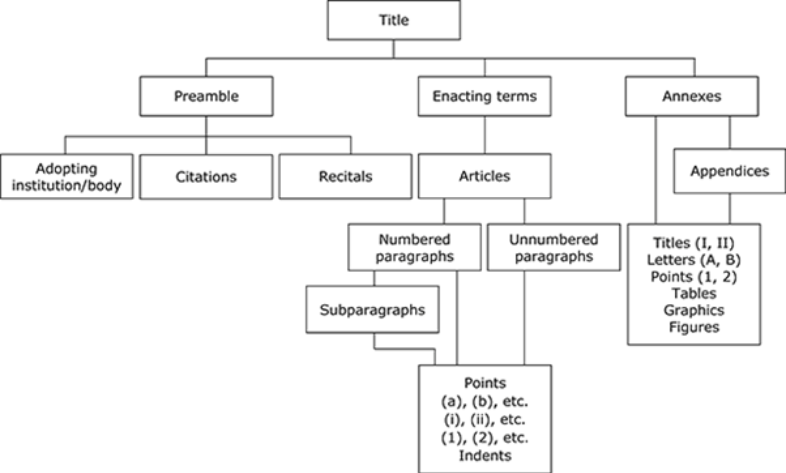
\includegraphics[width=0.8\textwidth]{Images/EU_doc_struct.png}
  \caption{Structure of an act \cite{eu_style_guide_2023}}
  \label{fig:euDocStruct}
\end{figure}

An article may contain several nested sub-levels, each of which can express a distinct legal requirement. To ensure that each requirement identified in this work can be traced to a unique and precise location in the legal text, the methodology preserves the complete supported hierarchy beneath an article. Figure~\ref{fig:article-sublevel-hierarchy} presents these possible sub-article levels and their containment relationships.

\begin{figure}[htbp]
    \centering
    \begin{forest}
        hierarchy
        [Article
            [Paragraph
                [Sub-Paragraph
                    [Point
                        [Point Sub-Paragraph]
                        [Sub-Point
                            [Indent]
                        ]
                    ]
                ]
                [Point
                    [Point Sub-Paragraph]
                    [Sub-Point
                        [Indent]
                    ]
                ]
            ]
        ]
    \end{forest}
    \caption{Supported containment hierarchy for sub-levels below an Article.
    Each connecting line denotes immediate containment.}
    \label{fig:article-sublevel-hierarchy}
\end{figure}


% #############################################################################
\section{Digital Operational Resilience Act}
Digital Operational Resilience is becoming more relevant as time progresses. Digital transactions are everywhere and financial services are used with increasing frequency trough digital means. This means that information and communication technology disruptions or attacks have the potential to cause financial instability, impacting both individual financial institutions as well as the entirety of the financial system.\cite{doraT}
This means that Digital Operational Resilience is of significant importance for the entire system.

\textit{Regulation (EU) 2022/2554 on digital operational resilience for
the financial sector}, in force since the 17\textsuperscript{th} of January 2025 is a \ac{EU} regulation primarily focused on ensuring financial entities manage risks arising from the use of \ac{ICT}. Due to the scope defined in Article 2, it applies to a wide range of financial entities and aims to create a uniform standard across the \ac{EU} trough the creation of a standardized regulatory framework\cite{doraT}. This is achieved by delineating precise criteria for \ac{ICT} risk management that financial institutions must comply with.

\begin{enumerate}
    \item \textbf{ICT Risk Management:}
    Financial entities must establish and maintain \ac{ICT} risk management frameworks to identify, detect, respond and recover from digital risks. This includes the creation of governance frameworks and procedures to effectively manage \ac{ICT} risks.

    The requirement placed by \ac{DORA} for financial institutions to have a strategy to recognize and reduce digital threats goes beyond conventional cybersecurity measures. It promotes the creation of resilient business continuity plans and advanced incident response mechanisms. The implementation of these measures ensures that financial institutions can sustain vital operations in the event of a cyber attack or digital disruption, reducing the impact on financial stability.\cite{doraT}
    \item \textbf{Incident Reporting:}
    \ac{DORA} requires the establishment of an effective incident management framework for reporting major \ac{ICT}-related incidents to authorities. This promotes a better understanding of emerging threats, enables a coordinated response and contributes to a shared comprehension of the \ac{ICT} risk environment. \cite{doraT}
    
    The purpose of implementing systematic incident reporting following \ac{DORA}'s guidelines is to promote transparency and collective vigilance. By promptly reporting significant \ac{ICT}-related incidents to relevant authorities, a coordinated approach to managing cyber threats is facilitated, enabling on-time interventions and the dissemination of critical threat intelligence across the sector. This information broadcast enhances the ability of financial institutions to withstand and recover from \ac{ICT} disruptions, but also bolsters overall stability and protection of the entire financial system.\cite{doraT}
    \item \textbf{Digital Operational Resilience Testing:}
    Testing under \ac{DORA} comprises both regular digital operational resilience testing and, for financial entities identified by their competent authority, advanced threat-led penetration testing (\ac{TLPT}). Regular testing is used to assess the institution's preparedness for \ac{ICT}-related incidents, identify weaknesses in digital operational resilience, and support the remediation of identified deficiencies. Testing is risk-based and includes both technical controls and the processes used to manage and respond to \ac{ICT} disruptions.\cite{doraT}

    In regard to regular testing frequency, \ac{DORA} states that ``financial entities, other than microenterprises, shall ensure, at least yearly, that appropriate tests are conducted on all \ac{ICT} systems and applications supporting critical or important functions.'' Other testing obligations, such as the testing of backup, restoration, recovery, and exit procedures, are subject to periodic or risk-based testing requirements.\cite{DORA}
    
    \ac{TLPT} is an advanced form of testing. It is required at least every three years for the non-micro financial entities identified by the competent authority. These tests should cover several or all critical or important functions of a financial entity and are performed on the relevant live production systems. They are based on the tactics, techniques, and procedures used by realistic threat actors in order to evaluate how well an organisation's resilience measures work against sophisticated cyber threats.\cite{DORA}
    
    Other types of regular tests are also mentioned, such as vulnerability assessments and scans, open source analyses, network security assessments, gap analyses, physical security reviews, questionnaires and scanning software solutions, source code reviews where feasible, scenario-based tests, compatibility testing, performance testing, end-to-end testing, and penetration testing.\cite{DORA}
    \item \textbf{Third-party Risk Management:}
    Recognizing the growing dependence on third-party service providers, \ac{DORA} mandates the implementation of rigorous management strategies to address \ac{ICT} risks that arise from outsourcing agreements in the supply chain, ensuring that financial entities have oversight over the resilience of their critical third-party providers. \cite{doraT}
    
    \ac{DORA}'s emphasis on the significance of adopting strategy for managing risks by applying the principles of operational resilience across the entire supply chain comes from the realization that a chain is only as strong as its weakest link. The dependence of financial institutions on external service providers (such as the cloud) has led to an increased risk of \ac{ICT} issues emerging from these given providers. By requiring that financial institutions enforce strict supervision and risk management protocols for their third-party vendors, \ac{DORA} is guaranteeing that these external collaborators comply with equivalent levels of digital resilience.\cite{doraT}
    
    \item \textbf{Oversight of critical \ac{ICT} third-party service providers:}
    In addition to requiring financial entities to manage \ac{ICT} third-party risk, \ac{DORA} establishes a Union-level Oversight Framework for critical \ac{ICT} third-party service providers. The European Supervisory Authorities, acting through their Joint Committee, designate providers as critical where:
    \begin{itemize}
        \item Their failure could have a systemic impact on the stability, continuity, or quality of financial services;
        \item They support critical or important functions;
        \item They are difficult to substitute.
    \end{itemize}  
    
    For each designated critical provider, a Lead Overseer is appointed from one of the European Supervisory Authorities. The Lead Overseer assesses the provider's \ac{ICT} risk-management arrangements, including security, availability, continuity, incident management, data portability, testing of \ac{ICT} systems and controls, and \ac{ICT} audits. It must also establish an annual oversight plan for the provider.
    
    The Lead Overseer may request relevant information and documentation, conduct investigations and on-site inspections, and issue recommendations concerning identified risks. Where a critical provider does not comply with requests for information, investigations, inspections, or required reports, the Lead Overseer may impose a periodic penalty payment of up to 1\% of the provider's average daily worldwide turnover.\cite{DORA}
    
    \item \textbf{Information Sharing:}
    \ac{DORA} encourages financial entities to share cyber threat intelligence and other relevant information to enhance collective understanding and defence mechanisms against \ac{ICT} threats.
    This collaboration creates a collective intelligence, strengthening the sector's overall ability to withstand \ac{ICT} threats.
    
    The use of this collective intelligence methodology allows entities to acquire knowledge from the experience of others, exchange optimal methods and work on more efficient strategies to manage digital risks. This collaboration is essential to improve the industry's capacity to adjust to the challenged presented in the current day and age.
\end{enumerate}

It is important to note that is work uses Regulation (EU) 2022/2554 (\ac{DORA}) as its sole binding legal source for the identification and traceability of regulatory requirements. \ac{RTS} and \ac{ITS} adopted under \ac{DORA}, including Commission Delegated Regulation (EU) 2024/1774, are outside the legal-analysis scope of this work. This decision limits the methodology to the primary obligations of the regulation and supports a focused assessment of stakeholder-specific regulatory impact.

%=======================================
% TEXT DOES NOT EXIST BELLOW THIS LEVEL 
%=======================================
\iffalse
\section{Comparative Architectural Summary}

The normative act analysed in this chapter,\ac{DORA} , enforces architectural constraints that shape the European digital landscape. When grouped together, and along with other legislative acts, these constraints form a complex web that is difficult to manage. To better manage this complexity, these regulations can be compared across three architecturally relevant dimensions that they share:
\begin{itemize}
    \item The object of the regulation or the entity of interest addressed by the law;
    \item The regulatory paradigm, meaning the legal nature and application of the constraints;
    \item The validation logic defining how assurance is established.
\end{itemize}

Each regulation and the corresponding values for each dimension can be found in table \ref{tab:normative_acts_comparison}. Following a per-dimension approach and beginning with the object of regulation, \ac{DORA} is sector-specific, focusing on financial institutions and their critical \ac{ICT} third-party service providers. In stark contrast, the \ac{CSA} targets the technical artifacts themselves instead of the entities producing those artifacts.

In terms of the regulatory paradigm, \ac{DORA} and \ac{CSA} are regulations, meaning they are ``binding in their entirety'' and uniformly applicable across all Member States. However, the \ac{CSA} is unique in its voluntary adoption. When entities choose to seek certification for their services, they must strictly adhere to the requirements in order to attain the desired certification level.

Lastly, regarding validation logic, \ac{DORA} introduces a proactive validation logic through regular reporting and testing procedures that include \ac{TLPT}s. The \ac{CSA} defines a structured certification logic, defining three distinct assurance levels that dictate cybersecurity risk and evaluation rigour.


\begin{table}[ht]
    \centering
    \renewcommand{\arraystretch}{1.8} % Increases row height for readability
    \begin{tabularx}{\textwidth}{l X X X}
        \hline
        \textbf{Act} & \textbf{Object of Regulation} & \textbf{Regulatory Paradigm} & \textbf{Validation Logic} \\
        \hline
        %\textbf{eIDAS2} & Identity \& Trust Services & Regulation & Mutual Recognition \\
        %\textbf{NIS2}   & Essential/Significant Entities & Directive & Supervision \& Liability \\
        \textbf{DORA}   & Financial Sector \& Supply Chain & Regulation & Resilience Testing (\ac{TLPT}) \& Systematic Reporting \\
        \textbf{CSA}    & \ac{ICT} Products and Services \& \ac{ENISA} & Regulation & Certification Levels \\
        \hline
    \end{tabularx}
    \caption{Comparison of the European Normative Acts addressed in this project}
    \label{tab:normative_acts_comparison}
\end{table}
\fi